49. $\cfrac{1}{3-x}\geqslant\cfrac{1}{(x^2-9)(3-x)}\Leftrightarrow\cfrac{-1}{(x-3)^2(x+3)}-\cfrac{1}{3-x}\leqslant0\Leftrightarrow
\cfrac{-1+x^2-9}{(x-3)^2(x+3)}\leqslant0\Leftrightarrow$\\$\cfrac{(x-\sqrt{10})(x+\sqrt{10})}{(x-3)^2(x+3)}\leqslant0.$\\ Применив метод интервалов, найдём ответ:
\begin{figure}[ht!]
\center{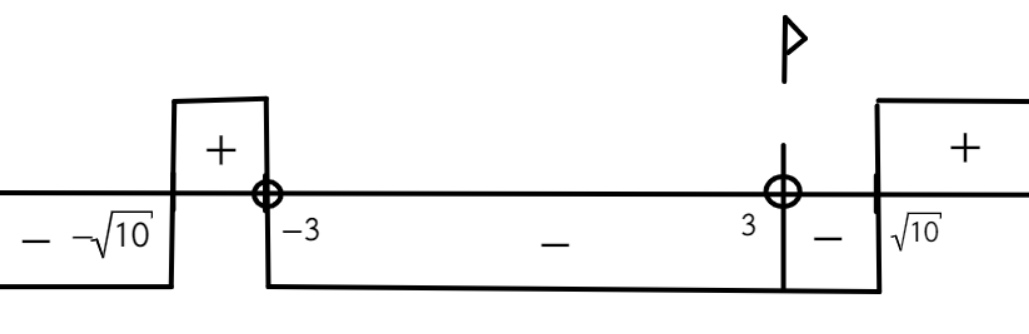
\includegraphics[scale=0.35]{int49.png}}
\end{figure}
$x\in(-\infty;-\sqrt{10}]\cup(-3;3)\cup(3;\sqrt{10}].$\\
